\chapter{경계 조건에서 열린 끈의 스펙트럼까지}

\lectureoverview{우리의 목표는 열린 끈을 양자화하고 그 상태를 입자라고 부를 수 있는지 판단하는 것이다. 접근법은 기초적이지만 만만치 않다. 먼저 \(0\leq\sigma\leq\pi\)에서 정의된 함수의 미적분과 푸리에 해석을 준비한다. 그런 다음 점처럼 보이는 성질 대신 입자 거동을 가르는 스펙트럼 기준을 도입하고, 횡방향 동역학이 비상대론적으로 바뀌는 무한 운동량 기술을 살펴본 뒤, 가벼운 질점들과 단단한 용수철들을 연결해 끈을 만든다. 연속 끈은 양 끝이 자유로운 파동계다. 이 계의 노이만 모드들은 진동수 \(1,2,3,\ldots\)를 갖는 조화 진동자들로 분리되므로, 양자화하면 간격이 벌어진 이산 스펙트럼이 생긴다. 마지막으로 끈의 상호작용은 열린 끈만으로는 충분하지 않음을 보여 준다. 열린 끈은 자기 양 끝을 이어 닫힌 끈이 될 수 있다.}

\section{열린 끈 구간에서의 미적분}

계산을 진행하다 보면 이산 합을 적분으로, 이웃한 점 사이의 차이를 미분으로 바꾸는 일이 반복된다. 이런 사실들을 물리학의 흐름을 끊기 전에 먼저 정리해 두는 편이 좋다.

\(x(\sigma)\)를

\begin{equation}
  0\leq \sigma\leq \pi .
\end{equation}

표기법에는 끈 이론의 의미가 담겨 있다. \(\sigma\)는 끈을 따라 잰 위치를 나타내고, \(x\)은 끈의 횡방향 좌표 가운데 하나가 된다. 구간을 \(N\)개의 조각으로 나누면

\begin{equation}
  \Delta\sigma=\frac{\pi}{N},
  \qquad
  \sigma_i=i\,\Delta\sigma,
  \qquad
  x_i=x(\sigma_i).
  \label{eq:l02-lattice}
\end{equation}

극한에서 함수가 매끄럽다면

\begin{equation}
  \Delta x_i\equiv x_i-x_{i-1}
  =
  \frac{\partial x}{\partial\sigma}\,\Delta\sigma
  +O\!\left((\Delta\sigma)^2\right),
  \label{eq:l02-difference}
\end{equation}

리만 합은 다음과 같이 된다.

\begin{equation}
  \sum_i x_i\,\Delta\sigma
  \longrightarrow
  \int_0^\pi x(\sigma)\,d\sigma .
  \label{eq:l02-riemann}
\end{equation}

\begin{figure}[H]
  \centering
  
\includegraphics[width=0.78\textwidth]{lecture_02_figure_01.png}
  \caption{나중에 연속체 극한을 취할 때 사용할 유한 차분과 리만 합의 규칙.}
  \lectureframe{00:04:20}
  \label{fig:l02-calculus-board}
\end{figure}

이들은 미적분에서 익히 아는 정의다. 여기서 중요한 것은 스케일링이다. \(\Delta x_i\)는 \(\Delta\sigma\)의 한 거듭제곱을 곱하고, 합은 적분으로 바뀔 때 역거듭제곱을 하나 곱한다.

\subsection{디리클레 및 노이만 경계 조건}

유한 구간에서 푸리에 해석을 하려면 먼저 양 끝에서 어떤 조건을 둘지 정해야 한다. 여기서 반복해서 사용할 조건은 두 가지다.

\begin{align}
  \text{Dirichlet:}\qquad
  &x(0)=x(\pi)=0,
  \label{eq:l02-dirichlet}\\
  \text{Neumann:}\qquad
  &\left.\partial_\sigma x\right|_{\sigma=0}
   =
   \left.\partial_\sigma x\right|_{\sigma=\pi}
   =0.
  \label{eq:l02-neumann}
\end{align}

양끝을 고정한 바이올린 줄은 디리클레 그림을 보여 준다. 경계에서 변위는 영이다. 노이만 함수는 경계에서 영일 필요가 없으며, 각 경계에서 기울기가 영이다. 두 가지 특징적인 모양을 칠판에서 함께 볼 수 있다.

\begin{figure}[H]
  \centering
  \begin{minipage}[t]{0.48\textwidth}
    \centering
    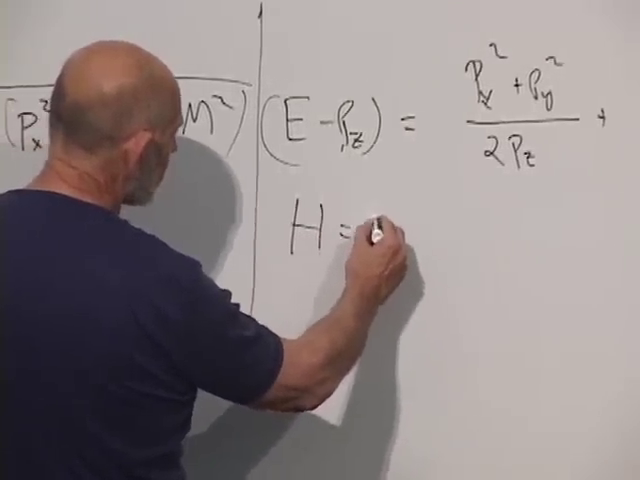
\includegraphics[width=\textwidth]{lecture_02_figure_02.png}
    \par\smallskip\footnotesize (a) 고정된 끝점과 기울기가 영인 끝점의 모양.
  \end{minipage}\hfill
  \begin{minipage}[t]{0.48\textwidth}
    \centering
    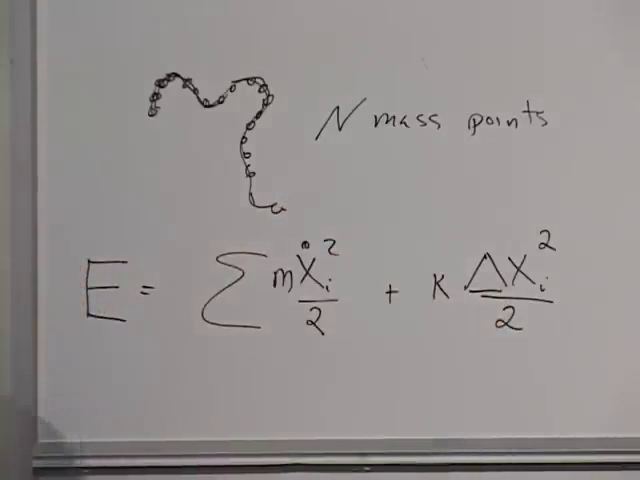
\includegraphics[width=\textwidth]{lecture_02_figure_03.png}
    \par\smallskip\footnotesize (b) 수직 막대를 따라 미끄러지는 가벼운 고리.
  \end{minipage}
  \caption{모양과 역학으로 나타낸 경계 조건. 고리가 미끄러지는 구조를 이용하면 자유 끝점의 횡방향 운동을 명확히 정의할 수 있다.}
  \lectureframe{00:08:50 and 00:12:15}
  \label{fig:l02-boundaries-board}
\end{figure}

\begin{figure}[H]
  \centering
  \begin{adjustbox}{max width=\linewidth}
  \begin{tikzpicture}[>=Latex,thick,scale=0.92]
    \begin{scope}
      \draw[->] (0,0) -- (4.4,0) node[right] {\(\sigma\)};
      \draw[->] (0,-1.25) -- (0,1.35) node[above] {\(x\)};
      \draw[blue!70!black]
        (0,0) .. controls (0.8,1.1) and (1.4,1.0) .. (2.0,0)
        .. controls (2.7,-1.0) and (3.4,-0.8) .. (4.1,0);
      \fill (0,0) circle (0.06);
      \fill (4.1,0) circle (0.06);
      \node at (2.05,-1.65) {Dirichlet: \(x=0\)};
    \end{scope}
    \begin{scope}[xshift=5.8cm]
      \draw[->] (0,0) -- (4.4,0) node[right] {\(\sigma\)};
      \draw[->] (0,-1.25) -- (0,1.35) node[above] {\(x\)};
      \draw[orange!85!black]
        (0,0.65) .. controls (0.8,0.65) and (1.1,-0.9) .. (2.0,-0.9)
        .. controls (2.9,-0.9) and (3.2,0.55) .. (4.1,0.55);
      \draw[orange!85!black] (0,0.65) -- (0.45,0.65);
      \draw[orange!85!black] (3.65,0.55) -- (4.1,0.55);
      \node at (2.05,-1.65) {Neumann: \(\partial_\sigma x=0\)};
    \end{scope}
  \end{tikzpicture}
  \end{adjustbox}
  \caption{디리클레 조건에서는 함수값이 고정되고, 노이만 조건에서는 기울기가 고정된다.}
  \label{fig:l02-boundaries-redraw}
\end{figure}

\begin{classroomqa}
\audiencequestion{열린 관이나 닫힌 관이 이 경계 조건 가운데 하나를 잘 보여 주는 예가 될까요?\lecturetimestamp{00:09:19}}
\lecturerresponse{그럴 수 있지만, 먼저 어떤 음향 변수를 전개하는지 밝혀야 한다. 압력 섭동과 종방향 변위는 열린 끝에서 서로 보완적인 이상화 조건을 따른다. 이 곁가지 질문을 칠판에서 결론내리기보다는 미끄럼 고리 모형을 사용하자. 질량이 거의 없는 고리는 막대를 따라 수직으로 움직일 수 있으므로, 끈의 끝은 자유롭고 노이만 조건이 직접 적용된다.}
\end{classroomqa}

\begin{classroomqa}
\audiencequestion{그래프가 수직으로 솟거나 날카로운 불연속을 가질 수 있나요?\lecturetimestamp{00:09:53}}
\lecturerresponse{푸리에 해석에서는 조각별 연속 함수에 고립된 불연속이 있어도 된다. 물리적인 끈에는 더 엄격한 조건이 필요하다. 불연속이 있으면 이웃한 점들이 끊어지고, 아래에서 유도할 연속체 에너지에서 공간 미분 \(\partial_\sigma x\)이 특이해진다. 따라서 함수 모양은 연속이고 미분 가능하다고 제한한다.}
\end{classroomqa}

\begin{classroomqa}
\audiencequestion{관의 열린 끝이나 다른 자유 끝점에도 왜 경계 조건이 있어야 하나요?\lecturetimestamp{00:11:14}}
\lecturerresponse{음향학의 예는 어떤 장을 택하느냐에 따라 달라지므로 토론에서 결론을 내리지 않았다. 역학의 예는 그렇지 않다. 매우 가벼운 고리는 자유롭게 미끄러질 수 있지만 줄의 마지막 구간에 연결되어 있다. 경계 조건을 가정하는 대신 뉴턴 법칙에서 유도하겠다. 끝점의 가속도가 유한하려면 기울기가 영이어야 한다.}
\end{classroomqa}

\subsection{푸리에 기저}

끝점의 조건을 정하면 그에 맞는 푸리에 기저도 정해진다. \(0\leq\sigma\leq\pi\)에서

\begin{align}
  x_D(\sigma)
  &=
  \sum_{n=1}^{\infty}x_n\sin(n\sigma),
  \label{eq:l02-dirichlet-series}\\
  x_N(\sigma)
  &=
  \sum_{n=0}^{\infty}x_n\cos(n\sigma).
  \label{eq:l02-neumann-series}
\end{align}

\eqref{eq:l02-dirichlet-series}의 모든 사인 함수는 양 끝점에서 0이 된다. \eqref{eq:l02-neumann-series}의 모든 코사인 함수는 끝점에서 미분값이 0이다. 하한이 서로 다른 데에는 이유가 있다. \(\sin(0\sigma)=0\)은 기여하지 않는 반면, \(\cos(0\sigma)=1\)는 상수 모드, 즉 영 모드다. 이 모드는 노이만 함수의 평균값을 나타낸다.

\begin{figure}[H]
  \centering
  \begin{minipage}[t]{0.48\textwidth}
    \centering
    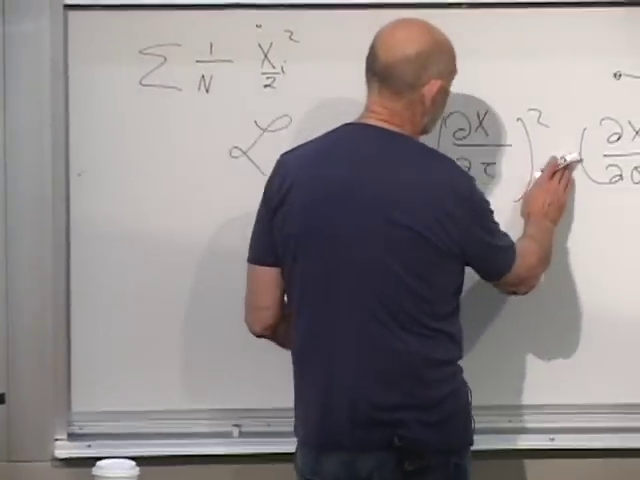
\includegraphics[width=\textwidth]{lecture_02_figure_04.png}
    \par\smallskip\footnotesize (a) 사인 및 코사인 전개.
  \end{minipage}\hfill
  \begin{minipage}[t]{0.48\textwidth}
    \centering
    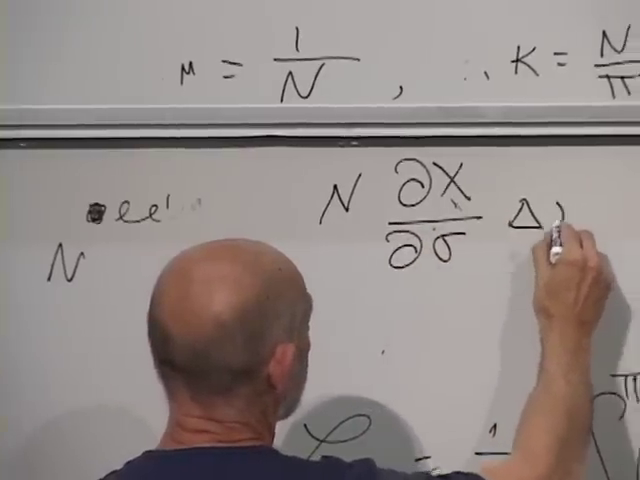
\includegraphics[width=\textwidth]{lecture_02_figure_05.png}
    \par\smallskip\footnotesize (b) 직교성과 예외적인 상수 모드.
  \end{minipage}
  \caption{줄의 모드를 대각화할 때 뒤에서 사용할 푸리에 성질.}
  \lectureframe{00:16:15 and 00:20:30}
  \label{fig:l02-fourier-board}
\end{figure}

미분하면 두 종류가 서로 바뀐다.

\begin{equation}
  \begin{aligned}
    \partial_\sigma\sin(n\sigma)&=n\cos(n\sigma),\\
    \partial_\sigma\cos(n\sigma)&=-n\sin(n\sigma).
  \end{aligned}
  \label{eq:l02-basis-derivatives}
\end{equation}

따라서 디리클레 급수를 미분하면 노이만 조건을 따르고, 노이만 급수를 미분하면 디리클레 조건을 따른다. 직교성 덕분에 서로 다른 모드 사이의 교차항은 사라진다.

\begin{align}
  \int_0^\pi\cos(n\sigma)\cos(m\sigma)\,d\sigma
  &=
  \frac{\pi}{2}\delta_{nm},
  && n,m\geq1,
  \label{eq:l02-cos-orthogonality}\\
  \int_0^\pi\sin(n\sigma)\sin(m\sigma)\,d\sigma
  &=
  \frac{\pi}{2}\delta_{nm},
  && n,m\geq1,
  \label{eq:l02-sin-orthogonality}\\
  \int_0^\pi 1\,d\sigma&=\pi .
  \label{eq:l02-zero-norm}
\end{align}

마지막 줄은 예외적인 \(n=m=0\) 코사인 노름이다. 상수는 영이 아닌 조화 모드와 같은 방식으로 정규화되지 않으며, 이 두 배 인자가 끈의 질량 중심 모드와 내부 모드를 구분해 준다.

\subsection{기억해 둘 진동자 공식 하나}

좌표를 재조정하여 역학적 질량을 1로 두면, 훅 법칙을 따르는 진동자는 다음과 같다.

\begin{align}
  E_{\mathrm{osc}}
  &=
  \frac12\dot q^{\,2}
  +\frac12\omega^2q^2,
  \label{eq:l02-oscillator-energy}\\
  L_{\mathrm{osc}}
  &=
  \frac12\dot q^{\,2}
  -\frac12\omega^2q^2.
  \label{eq:l02-oscillator-lagrangian}
\end{align}

\begin{figure}[H]
  \centering
  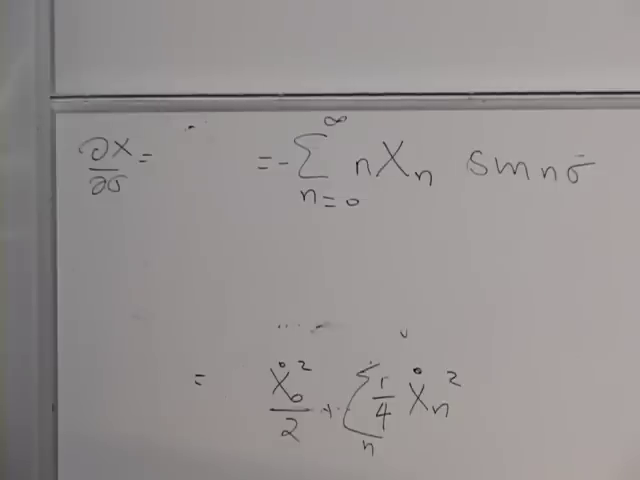
\includegraphics[width=0.68\textwidth]{lecture_02_figure_06.png}
  \caption{계수에서 \(q^2\)을 보면 \(\omega^2\)를 바로 알 수 있도록 쓴 진동자의 에너지.}
  \lectureframe{00:24:00}
  \label{fig:l02-oscillator-board}
\end{figure}

고전적으로는 \(\omega=\sqrt{\kappa/m}\)이다. 좌표를 재조정하여 \(m=1\)로 두었다. 양자역학에서는

\begin{equation}
  E_Q=\hbar\omega\left(Q+\frac12\right),
  \qquad Q=0,1,2,\ldots .
  \label{eq:l02-oscillator-spectrum}
\end{equation}

준위 간격만 볼 때는 모든 준위에 공통으로 들어가는 바닥 상태 항을 빼고, 각 양자가 \(\hbar\omega\)의 에너지를 갖는다고 말할 수 있다. 끈 계산도 처음에는 정확히 그렇게 하고, 전체 영점 에너지는 나중으로 미룬다.

\begin{classroomqa}
\audiencequestion{에너지 식에서 진동수는 어떻게 읽어 내나요?\lecturetimestamp{00:23:21}}
\lecturerresponse{재척도화하기 전에는 \(\omega=\sqrt{\kappa/m}\)이다. 단위질량으로 두면 퍼텐셜 항은 \(\frac12\omega^2q^2\)이므로, 이차항의 계수는 진동수의 제곱이다.}
\end{classroomqa}

\section{복합계가 입자가 되는 기준은 무엇인가?}

끈은 길게 뻗은 물체이며, 여러 조각이 서로 결합한 계로 모형화할 것이다. 그렇다면 그 양자 상태를 어떤 의미에서 입자라고 할 수 있을까? 점처럼 보이는지가 결정적인 기준일 수는 없다. 양성자와 중성자는 복합 입자다. 전자와 광자도 고유한 내부 구조가 확인된 적은 없지만 양자장의 드레싱을 동반한다. 아무것도 둘러싸지 않은 고전적 기하학적 점은 양자 들뜸을 그리는 적절한 그림이 아니다.

질량과 질량중심 위치만으로도 충분하지 않다. 밀폐된 기체 상자에도 둘 다 있다. 커피 잔에도 둘 다 있다. 보통 어느 쪽도 입자라고 부르지 않는다. 쪼갤 수 없어야 한다는 조건도 맞지 않는다. 양성자는 쪼갤 수 있고, 스핀 역시 미시적 입자와 거시적 물체를 구분해 주지 않는다.

유용한 기준은 스펙트럼상 고립되어 있는지 여부다. 수직축에 정지 에너지를 놓고 내부의 다른 상태에 도달하는 데 에너지가 얼마나 필요한지 살펴보자. 전자에는 그 바로 위에 실험적으로 접근할 수 있는 전자 들뜸 상태의 탑이 없다. 양성자에는 공명 상태가 있지만, 가장 낮은 상태에 도달하는 데 수백 MeV가 필요하다. 이는 양성자 질량의 상당 부분이다. 그 상태들은 서로 충분히 떨어져 있어 각각 식별할 수 있다.

커피 잔은 정반대다. 장파장 음향 모드에 임의로 작은 에너지를 더하거나, 분자를 살짝 흔들거나, 포논 하나를 만들 수 있다. 아주 좁은 에너지 구간에 어마어마하게 많은 상태가 빽빽이 들어 있다. 실험실 규모에서는 이들이 연속체를 이룬다. 이것이 입자와 \emph{잡다한 물질}을 실질적으로 구분하는 기준이다.

\begin{figure}[H]
  \centering
  \includegraphics[width=0.58\textwidth]{lecture_02_figure_07.png}
  \caption{보통 물질의 빽빽한 들뜸 상태와 고립된 입자 준위를 비교할 때 칠판에 그린 수직 에너지축.}
  \lectureframe{00:31:10}
  \label{fig:l02-spectrum-board}
\end{figure}

\begin{figure}[H]
  \centering
  \begin{adjustbox}{max width=\linewidth}
  \begin{tikzpicture}[>=Latex,thick]
    \begin{scope}
      \draw[->] (0,0) -- (0,4.8) node[above] {energy};
      \draw[blue!70!black,line width=1.2pt] (-1.0,0.65) -- (1.0,0.65);
      \draw[blue!70!black,line width=1.2pt] (-1.0,3.65) -- (1.0,3.65);
      \node[right] at (1.05,0.65) {ground state};
      \node[right] at (1.05,3.65) {first internal excitation};
      \draw[<->] (0.65,0.75) -- (0.65,3.55)
        node[midway,right] {large gap};
      \node at (0,-0.55) {particle-like};
    \end{scope}
    \begin{scope}[xshift=7.0cm]
      \draw[->] (0,0) -- (0,4.8) node[above] {energy};
      \foreach \y in {0.55,0.69,0.82,0.94,1.05,1.15,1.24,1.32,1.39,1.45,
        1.51,1.57,1.63,1.70,1.78,1.87,1.97,2.09,2.22,2.36,2.51,2.67,2.84,
        3.02,3.21,3.41,3.62,3.84,4.07}
        \draw[orange!85!black] (-0.95,\y) -- (0.95,\y);
      \node[right] at (1.05,2.25) {dense phonon and internal states};
      \node at (0,-0.55) {macroscopic matter};
    \end{scope}
  \end{tikzpicture}
  \end{adjustbox}
  \caption{강의에서 사용하는 조작적 입자 기준은 문자 그대로 점처럼 보이는지가 아니라 스펙트럼상 고립되어 있는지 여부다.}
  \label{fig:l02-particle-redraw}
\end{figure}

이 기준을 적용하면 철학적 질문을 계산 문제로 바꿀 수 있다. 끈을 양자화하고 내부 에너지 준위를 찾아 그 간격을 살펴보자. 끈의 첫 들뜸 상태가 플랑크 규모에 있고 관측되는 바닥 상태는 가볍다면, 그 간격은 현재 가속기가 도달하는 에너지보다 20자릿수 넘게 크다. 따라서 접근 가능한 모든 에너지 영역에서 끈은 기본 입자처럼 거동한다.

\begin{classroomqa}
\audiencequestion{입자처럼 보이는 성질은 관측 규모의 문제일 뿐인가요? 충분히 확대하면 준위들이 더 이상 분리되어 있지 않게 되나요?\lecturetimestamp{00:33:33}}
\lecturerresponse{확대하면 물체가 여러 구성 요소로 이루어져 있음을 알아낼 수 있지만, 스펙트럼이 사라지는 것은 아니다. 중요한 비교 대상은 실험의 에너지 분해능과 첫 내부 들뜸 상태까지의 간격이다. 그 간격이 엄청나게 크면 복합 물체도 계속 입자처럼 거동할 수 있다.}
\end{classroomqa}

\begin{classroomqa}
\audiencequestion{보통 바이올린 줄은 왜 입자가 아닌가요?\lecturetimestamp{00:34:37}}
\lecturerresponse{진동 양자 하나의 에너지는 거시적인 줄의 정지 에너지와 비교하면 측정할 수 없을 만큼 작다. 그러므로 아주 좁은 상대적 에너지 구간에도 양자 상태가 많이 들어간다. 이 줄은 스펙트럼 비교에서 고립된 쪽이 아니라 빽빽한 쪽에 속한다.}
\end{classroomqa}

\begin{classroomqa}
\audiencequestion{양자장이 가상 요동으로 둘러싸고 있어도 광자와 전자는 점입자인가요?\lecturetimestamp{00:35:40}}
\lecturerresponse{\emph{점}이라는 고전적 단어가 너무 많은 일을 떠맡고 있다. 물리적인 전자와 광자는 드레싱된 장의 들뜸 상태지만, 실험에서 어느 쪽도 고유한 구성 요소 구조나 유한한 형상 인자를 보인 적은 없다. 여기서 중요한 것은 둘 다 거의 축퇴된 내부 상태들이 빽빽이 이어지는 탑을 갖지 않는다는 점이다.\editorialnote{강의에서는 전자의 이상 자기 모멘트를 측정 가능한 양자적 퍼짐과 연결한다. 현대적 용어로 이상 자기 모멘트는 복사 드레싱 효과이지, 유한한 전자 반지름이 확인되었다는 증거가 아니다. 통상 점처럼 보인다는 말은 시험한 규모까지 고유한 내부 구조나 형상 인자가 검출되지 않았다는 뜻이다.}}
\end{classroomqa}

\begin{classroomqa}
\audiencequestion{광자의 크기는 진동수에 따라 달라지나요?\lecturetimestamp{00:36:49}}
\lecturerresponse{파장은 분명히 달라진다. 하지만 이는 고유한 구성 요소의 크기와는 다르다. 진동수를 바꾸면 파동 묶음과 파장이 달라질 뿐, 광자의 내부 반지름이 확인되는 것은 아니다.}
\end{classroomqa}

\section{큰 운동량에서의 정확한 횡방향 역학}

이제 상대론적 어려움으로 돌아가자. 빠르게 회전하는 곤봉은 질량중심을 정지시킨다고 해서 비상대론적으로 다룰 수 없다. 양 끝은 여전히 서로에 대해 상대론적으로 움직인다. 비상대론적 근사가 성립하지 않는 까닭은 내부의 상대 운동에 있다.

하지만 다른 극한이 있다. \(z\)축을 정하고, 계 전체를 아주 큰 양의 종방향 운동량 \(P_z\)을 갖도록 로런츠 변환한다. 횡방향 운동량은

\begin{equation}
  p_\perp^2=p_x^2+p_y^2
\end{equation}

유한하게 유지한다. 그러면 로런츠 변환 전의 내부 운동이 상대론적이었더라도 \(P_z\to\infty\) 극한에서 횡방향 투영은 정확히 비상대론적 해밀토니안 형태를 갖는다.

\begin{classroomqa}
\audiencequestion{무한 운동량은 질량을 가진 계가 실제로 빛의 속도에 도달한다는 뜻인가요?\lecturetimestamp{00:40:43}}
\lecturerresponse{유한한 로런츠 변환으로는 빛의 속도에 도달하지 못한다. \(P_z\)이 임의로 커질 때 잘 정의된 극한을 갖는 양들을 구성한다. 이 표현은 극한을 취하는 절차를 가리키며, \(v=c\)인 유한한 물리적 상태를 뜻하지 않는다.}
\end{classroomqa}

\begin{classroomqa}
\audiencequestion{어느 축을 택해야 하나요? 물체가 그 축을 중심으로 회전하거나 그 축을 가로질러 회전한다면 어떻게 되나요?\lecturetimestamp{00:41:14}}
\lecturerresponse{어느 축이든 택해도 되고, 계 전체를 그 축 방향으로 로런츠 변환하면 된다. 명시적으로 역학을 다루는 부분은 그 축에 수직인 평면으로의 투영이다. 회전하는 막대는 짧아져 보이거나 그 평면을 가로질러 쓸고 지나갈 수 있지만, 횡방향 투영은 비상대론적 형태를 갖는다.}
\end{classroomqa}

끈에는 이 표현을 특히 강력하게 만드는 성질이 하나 더 있다. 광전면 게이지에서는 종방향 내부 좌표가 독립적인 진동자가 아니다. 구속 조건에 따라 이 좌표들은 횡방향 운동으로부터 결정된다. 따라서 물리적 자유도를 복원하는 데 횡방향 끈만 알면 충분하다.

\begin{classroomqa}
\audiencequestion{독립적인 종방향 좌표가 없다는 말은 끈이 그저 얇은 샌드위치 안에 갇혀 있다는 뜻인가요?\lecturetimestamp{00:42:26}}
\lecturerresponse{로런츠 수축 때문에 로런츠 변환된 계에서 종방향 길이가 짧아지는 것은 맞지만, 그보다 더 강한 내용이다. 남아 있는 종방향 운동은 횡방향 운동에 의해 구속되므로 독립적으로 지정할 수 없다.}
\end{classroomqa}

\begin{classroomqa}
\audiencequestion{횡방향 자료로 줄이는 것이 홀로그래피 원리와 관련이 있나요?\lecturetimestamp{00:43:12}}
\lecturerresponse{홀로그래피 개념으로 이어진 사고의 흐름과 밀접하게 관련되어 있지만, 그 연결을 더 살펴보면 지금 계산에서 벗어나게 된다. 여기서는 횡방향 끈만 다루어도 된다는 점을 뒷받침하는 데에만 이 사실을 사용한다.}
\end{classroomqa}

\subsection{로런츠 변환 항을 빼고 시간을 재조정하기}

구성 입자의 질량, 운동 에너지, 결합 에너지를 모두 포함한 계 전체의 불변 질량을 \(M\)이라 하자. 단위 \(c=1\)에서는

\begin{equation}
  E=\sqrt{P_z^2+p_\perp^2+M^2}.
  \label{eq:l02-relativistic-energy}
\end{equation}

\(P_z\)이 \(p_\perp\)와 \(M\)보다 훨씬 크면

\begin{equation}
  E
  =
  P_z+\frac{p_\perp^2+M^2}{2P_z}
  +O(P_z^{-3}).
  \label{eq:l02-large-pz}
\end{equation}

\begin{figure}[H]
  \centering
  \includegraphics[width=0.76\textwidth]{lecture_02_figure_08.png}
  \caption{횡방향 운동량과 불변 질량을 유지한 채 전개한 큰 \(P_z\) 전개식.}
  \lectureframe{00:47:30}
  \label{fig:l02-large-pz-board}
\end{figure}

선도항은 크지만 내부 상태에 관한 정보는 담고 있지 않다. 부스트된 원자가 전체 종방향 운동량은 바꾸지 않은 채 내부 준위 사이에서 전이하는 경우처럼 \(P_z\)을 보존하는 과정에서는 이 항이 모든 에너지 차이에서 상쇄된다. 따라서 다음을 살펴보자.

\begin{equation}
  E-P_z=\frac{p_\perp^2+M^2}{2P_z}+O(P_z^{-3}).
  \label{eq:l02-residual-energy}
\end{equation}

분모에는 물리적 의미가 있다. 해밀토니안이 시간 변화를 생성하므로, 작은 잔류 에너지는 내부의 시간 변화가 실험실 시간으로는 느리게 보인다는 뜻이다. 이것이 시간 지연이다. 내부 운동을 유지하려면 재조정된 진화 매개변수 \(\tau\)를 도입하거나, 이와 동등하게 잔류 해밀토니안을 \(P_z\)배 한다.

\begin{equation}
  H_\perp
  \equiv
  \lim_{P_z\to\infty}P_z(E-P_z)
  =
  \frac12p_\perp^2+\frac12M^2.
  \label{eq:l02-transverse-hamiltonian}
\end{equation}

\begin{figure}[H]
  \centering
  \begin{minipage}[t]{0.48\textwidth}
    \centering
    \includegraphics[width=\textwidth]{lecture_02_figure_09.png}
    \par\smallskip\footnotesize (a) \(H=i\partial_t\)와 느려진 내부 시간 변화.
  \end{minipage}\hfill
  \begin{minipage}[t]{0.48\textwidth}
    \centering
    \includegraphics[width=\textwidth]{lecture_02_figure_10.png}
    \par\smallskip\footnotesize (b) 시간 재척도화 뒤의 유한한 횡방향 해밀토니안.
  \end{minipage}
  \caption{시간 지연된 잔여 에너지에서 유한한 2차원 해밀토니안으로.}
  \lectureframe{00:49:20 and 00:52:40}
  \label{fig:l02-lightfront-board}
\end{figure}

이는 2차원에서 움직이는 단위 질량 입자의 형태와 정확히 같다. 운동 에너지는 \(p_\perp^2/2\)이고 내부 에너지는 \(M^2/2\)이다. 특이한 점은 제곱이 들어간다는 것이다. 이 기술에서 정지 에너지 또는 결합 에너지의 역할을 하는 양은 불변 질량의 제곱에 비례한다.\editorialnote{통상적인 빛전면 변수 \(P^\pm=(E\pm P_z)/\sqrt2\)를 쓰면 정확한 질량 껍질 관계는 \(2P^+P^-=p_\perp^2+M^2\)이다. 식 \eqref{eq:l02-transverse-hamiltonian}은 같은 불변 관계를 강의에서 사용한 큰 \(P_z\) 정규화로 나타낸 것이다.}

\begin{classroomqa}
\audiencequestion{복합계의 각 부분이 가진 종방향 운동량은 어떻게 되었나요?\lecturetimestamp{00:51:30}}
\lecturerresponse{일반적인 복합 물체에서는 각 구성 요소가 전체 \(P_z\)의 어느 분율을 갖는지 유지해야 한다. 위 공식은 전체 질량중심 운동량을 사용한다. 끈 이론은 구속 조건에 따라 상대적 종방향 운동이 횡방향 자유도로부터 결정된다는 점에서 특별하다. 따라서 독립적인 종방향 진동자를 더할 필요가 없다.}
\end{classroomqa}

\section{이산적인 열린 끈}

이제 로런츠 변환된 끈은 횡방향 평면에서만 명시적으로 움직인다. 두 좌표를 \(X\)와 \(Y\)이라 하고, 우선 이를 \(N\)개의 질점과 \(N-1\)개의 용수철을 연결한 모형으로 근사하자. 각 점의 유사 질량이 \(\mu\)이고 이웃한 점 사이 용수철의 용수철 상수가 \(k\)라면 에너지는 다음과 같다.

\begin{equation}
  E_N
  =
  \sum_i
  \left[
    \frac{\mu}{2}
    \left(\dot X_i^2+\dot Y_i^2\right)
    +
    \frac{k}{2}
    \left((\Delta X_i)^2+(\Delta Y_i)^2\right)
  \right].
  \label{eq:l02-discrete-energy}
\end{equation}

모든 \(X\) 항에는 횡방향 평면이 두 방향을 가지므로 같은 형태의 \(Y\) 항이 있다. 첨자 \(i\)는 사슬을 따라 놓인 점을 가리키며, 공간 좌표가 아니다.

\begin{figure}[H]
  \centering
  \begin{minipage}[t]{0.48\textwidth}
    \centering
    \includegraphics[width=\textwidth]{lecture_02_figure_11.png}
    \par\smallskip\footnotesize (a) 구슬 사슬과 그 이산 에너지.
  \end{minipage}\hfill
  \begin{minipage}[t]{0.48\textwidth}
    \centering
    \includegraphics[width=\textwidth]{lecture_02_figure_12.png}
    \par\smallskip\footnotesize (b) \(N\)이 커질 때 \(\mu\)와 \(k\)의 스케일링.
  \end{minipage}
  \caption{연속체 극한을 취하기 전의 조절된 열린 줄.}
  \lectureframe{00:57:42 and 01:02:40}
  \label{fig:l02-chain-board}
\end{figure}

\begin{figure}[H]
  \centering
  \begin{adjustbox}{max width=\linewidth}
  \begin{tikzpicture}[>=Latex,thick]
    \foreach \i in {0,...,8} {
      \coordinate (p\i) at ({1.05*\i},{0.30*sin(55*\i)});
      \filldraw[white] (p\i) circle (0.10);
      \draw (p\i) circle (0.10);
    }
    \foreach \i in {0,...,7} {
      \pgfmathtruncatemacro{\j}{\i+1}
      \draw[decorate,decoration={zigzag,segment length=4pt,amplitude=2pt}]
        (p\i) -- (p\j);
    }
    \node[above=0.35cm of p0] {\(i=0\)};
    \node[above=0.35cm of p8] {\(i=N-1\)};
    \draw[<->] (0,-1.15) -- (8.4,-1.15)
      node[midway,below] {\(0\leq\sigma\leq\pi\)};
    \node at (4.2,1.25)
      {\(\mu=1/N,\quad k=N/\pi^2,\quad\Delta\sigma=\pi/N\)};
  \end{tikzpicture}
  \end{adjustbox}
  \caption{명확한 정규화 모형이다. 사슬을 더 잘게 나누면 점은 가벼워지고 미시적 용수철은 더 단단해진다.}
  \label{fig:l02-chain-redraw}
\end{figure}

매개변수 \(\sigma\)는 사슬을 따라 잰 위치를 나타낸다. \(0\leq\sigma\leq\pi\)로 두는 것은 관례일 뿐, 물리적 길이를 측정하는 것이 아니다. 이는 끈에 두 끝점이 있음을 상기시킨다. 나중에 닫힌 끈은 \(0\leq\sigma<2\pi\)에서 주기적으로 매개화할 것이다.

연속체 극한에서도 계 전체의 역학이 유한하게 유지되어야 한다. 구슬 하나의 질량을 고정하면 유사 총질량이 발산하므로 다음과 같이 둔다.

\begin{equation}
  \mu=\frac{1}{N}.
  \label{eq:l02-mu-scaling}
\end{equation}

그러면 \(N\mu=1\)이다. 이는 상대론적 정지 질량 \(M\)이 아니라 횡방향 유사 모형에서 관성 계수로 쓰이는 양이다.

용수철을 직렬로 연결하면 개수가 늘어날수록 전체가 더 부드러워진다. 사슬 전체의 강성을 유한하게 유지하려면 각 미시적 용수철은 더 단단해져야 한다.

\begin{equation}
  k=\frac{N}{\pi^2}
  =\frac{1}{\pi\,\Delta\sigma}.
  \label{eq:l02-k-scaling}
\end{equation}

필요한 조건은 \(k\propto N\)뿐이다. \(\pi^2\) 인자는 연속체 공식에 불필요한 \(\pi\) 인자가 남지 않도록 선택한 정규화다.

\begin{classroomqa}
\audiencequestion{\(\mu\)는 끈의 각 점이 갖는 물리적 정지 질량인가요?\lecturetimestamp{01:10:34}}
\lecturerresponse{아니다. 횡방향 사슬에 등장하는 비상대론적 유사 질량이다. 이를 \(M\)라고 부르면 상대론적 끈 상태 전체의 불변 정지 질량과 혼동하게 된다. 지금은 올바른 연속체 관성을 얻는 역할만 한다.}
\end{classroomqa}

\section{연속체 파동계}

처음에 마련한 규칙을 적용하자. \(1/N=\Delta\sigma/\pi\)이므로,

\begin{align}
  \sum_i\frac{\mu}{2}\dot X_i^2
  &=
  \frac{1}{2\pi}
  \sum_i\dot X_i^2\,\Delta\sigma
  \longrightarrow
  \frac{1}{2\pi}
  \int_0^\pi
  \left(\partial_\tau X\right)^2d\sigma ,
  \label{eq:l02-kinetic-limit}\\
  \sum_i\frac{k}{2}(\Delta X_i)^2
  &\longrightarrow
  \frac{1}{2\pi}
  \int_0^\pi
  \left(\partial_\sigma X\right)^2d\sigma .
  \label{eq:l02-potential-limit}
\end{align}

두 번째 줄에는 \(\Delta X_i=\partial_\sigma X\,\Delta\sigma\)과 \(k=1/(\pi\Delta\sigma)\)을 사용한다. \(Y\)에도 같은 계산이 적용된다.

\begin{figure}[H]
  \centering
  \begin{minipage}[t]{0.48\textwidth}
    \centering
    \includegraphics[width=\textwidth]{lecture_02_figure_13.png}
    \par\smallskip\footnotesize (a) 합을 적분으로, 차분을 도함수로 바꾸기.
  \end{minipage}\hfill
  \begin{minipage}[t]{0.48\textwidth}
    \centering
    \includegraphics[width=\textwidth]{lecture_02_figure_14.png}
    \par\smallskip\footnotesize (b) 완성된 연속체 에너지.
  \end{minipage}
  \caption{이산 사슬에서 \(\sigma\) 구간 위의 장으로.}
  \lectureframe{01:05:40 and 01:07:00}
  \label{fig:l02-continuum-board}
\end{figure}

그 결과 얻는 에너지와 라그랑지안은 다음과 같다.

\begin{align}
  E
  &=
  \frac{1}{2\pi}
  \int_0^\pi d\sigma\,
  \left[
    (\partial_\tau X)^2+(\partial_\tau Y)^2\right.\notag\\[-0.25em]
  &\hspace{6.5em}\left.
    +(\partial_\sigma X)^2+(\partial_\sigma Y)^2
  \right],
  \label{eq:l02-continuum-energy}\\
  L
  &=
  \frac{1}{2\pi}
  \int_0^\pi d\sigma\,
  \left[
    (\partial_\tau X)^2+(\partial_\tau Y)^2\right.\notag\\[-0.25em]
  &\hspace{6.5em}\left.
    -(\partial_\sigma X)^2-(\partial_\sigma Y)^2
  \right].
  \label{eq:l02-continuum-lagrangian}
\end{align}

\begin{figure}[H]
  \centering
  \includegraphics[width=0.78\textwidth]{lecture_02_figure_15.png}
  \caption{운동 항과 신축 항이 서로 반대 부호를 갖는 연속체 라그랑지안.}
  \lectureframe{01:08:48}
  \label{fig:l02-lagrangian-board}
\end{figure}

\(\sigma\)을 보통의 공간 좌표로, \(X\)를 장 \(\phi\)로 바꾸어 쓰면 이는 1차원 파동장의 에너지와 라그랑지안이다. \eqref{eq:l02-continuum-lagrangian}을 변분하면 다음을 얻는다.

\begin{equation}
  \left(\partial_\tau^2-\partial_\sigma^2\right)X=0,
  \qquad
  \left(\partial_\tau^2-\partial_\sigma^2\right)Y=0.
  \label{eq:l02-wave-equation}
\end{equation}

지금까지의 논증에서 이 방정식들을 직접 풀 필요는 없다. 파동이 끈을 따라 좌우로 이동하고 끝점에서 반사된다고 생각하면 된다. 디리클레 조건에서 반사되면 변위의 부호가 뒤집히고, 노이만 조건에서 반사되면 부호가 유지된다.

\begin{classroomqa}
\audiencequestion{\(\tau\)는 정확히 어떤 시간 변수인가요?\lecturetimestamp{01:08:54}}
\lecturerresponse{큰 \(P_z\) 기술에서 내부 운동을 추적하기 위해 사용하는 재조정된 시간이다. 계와 함께 로런츠 변환된 시계는 실험실 시간에 비해 느리게 간다. \(\tau\)는 이 시간 지연을 없애 내부 진동이 유한한 속도를 유지하도록 한다. 이 횡방향 역학에서는 단순히 시간으로 다룰 수 있다.\editorialnote{강의에서는 비격식적으로 \(\tau\)를 고유 시간이라고 부른다. 뻗어 있는 끈에서 정확한 광전면 진화 매개변수는 게이지를 고정해 재조정한 시간이지, 모든 점이 공유하는 하나의 불변 고유 시간은 아니다. 시간 지연에 관한 논증은 달라지지 않는다.}}
\end{classroomqa}

횡방향 평면에서 질량중심이 정지해 있을 때, \eqref{eq:l02-continuum-energy}의 내부 항은 \eqref{eq:l02-transverse-hamiltonian}의 정규화에 따라 \(M^2\)에 비례한다. 그래서 겉보기에는 평범한 이 파동계를 양자화하면 상대론적 질량 스펙트럼이 드러난다.

\begin{classroomqa}
\audiencequestion{\(P_z(E-P_z)\)에는 이름이 있나요?\lecturetimestamp{01:11:00}}
\lecturerresponse{보통 광원뿔 에너지 또는 광전면 에너지라고 부른다. 광전면이라는 이름이 진화면으로 사용하는 영공간을 더 잘 나타낸다. 전통적인 용어는 계산에 중요하지 않다.}
\end{classroomqa}

\begin{classroomqa}
\audiencequestion{여기서 말하는 원뿔은 보통 시공간의 광원뿔을 뜻하나요? 이 용어는 디랙이 도입했나요?\lecturetimestamp{01:11:17}}
\lecturerresponse{영좌표 구성은 45도 축으로 그릴 수 있지만, 여기서 진화면은 완전히 펼쳐지는 원뿔이 아니라 광전면이다. 디랙은 관련된 상대론적 동역학 형식들을 발전시켰다. 누가 역사적으로 이 이름을 붙였는지는 결론내리지 않았으며, 방정식에는 영향을 주지 않는다.}
\end{classroomqa}

\section{자유단이 노이만 조건을 따르는 이유}

이제 끝점 조건을 가정하지 않고 유도할 수 있다. 로런츠 변환된 횡방향 역학은 정확히 비상대론적 형태이므로 뉴턴 법칙을 적용해도 된다. 내부의 질점에는 양쪽 용수철이 힘을 가한다. 마지막 점에는 이웃한 점과 연결하는 용수철 하나만 힘을 가한다.

\begin{classroomqa}
\audiencequestion{상대론적 끈을 논하면서 어떻게 뉴턴 법칙을 사용할 수 있나요?\lecturetimestamp{01:14:52}}
\lecturerresponse{로런츠 변환하지 않은 시공간 운동 전체에 뉴턴 역학을 적용하는 것은 아니다. 무한 운동량 기술에서 횡방향 변수에 적용하는 것이다. 이 변수들의 해밀토니안은 정확히 비상대론적 형태를 갖는다.}
\end{classroomqa}

오른쪽 끝점에서 훅 법칙을 적용하면, 방향에 따른 부호를 제외하고 다음을 얻는다.

\begin{equation}
  F_{\mathrm{end}}
  =
  -k\,\Delta X
  =
  -\frac{1}{\pi\Delta\sigma}
   \left(\partial_\sigma X\,\Delta\sigma\right)
  =
  -\frac{1}{\pi}\partial_\sigma X .
  \label{eq:l02-endpoint-force}
\end{equation}

\begin{figure}[H]
  \centering
  \begin{minipage}[t]{0.48\textwidth}
    \centering
    \includegraphics[width=\textwidth]{lecture_02_figure_16.png}
    \par\smallskip\footnotesize (a) 국소 기울기에 비례하는 끝점 힘.
  \end{minipage}\hfill
  \begin{minipage}[t]{0.48\textwidth}
    \centering
    \includegraphics[width=\textwidth]{lecture_02_figure_17.png}
    \par\smallskip\footnotesize (b) 유한 가속도 조건.
  \end{minipage}
  \caption{자유 끝점 경계 조건을 뉴턴 법칙에서 유도하기.}
  \lectureframe{01:18:20 and 01:20:10}
  \label{fig:l02-neumann-board}
\end{figure}

마지막 점에 대한 뉴턴 방정식은 다음과 같다.

\begin{equation}
  \mu\,\partial_\tau^2X=F_{\mathrm{end}},
  \qquad
  \mu=\frac1N=\frac{\Delta\sigma}{\pi}.
  \label{eq:l02-endpoint-newton}
\end{equation}

\eqref{eq:l02-endpoint-force}과 \eqref{eq:l02-endpoint-newton}를 결합하면

\begin{equation}
  \partial_\sigma X
  =
  -\Delta\sigma\,\partial_\tau^2X
  \quad\text{at the right endpoint},
  \label{eq:l02-endpoint-scaling}
\end{equation}

왼쪽 끝점에서는 힘의 부호가 반대다. \(\partial_\sigma X\)이 영이 아닌 상수에 가까워지는 한편 \(\Delta\sigma\to0\)이면 끝점 가속도는 \(N\)에 비례해 발산한다. 따라서 가속도가 유한한 타당한 연속체 극한을 얻으려면 다음이 필요하다.

\begin{equation}
  \left.\partial_\sigma X\right|_{0,\pi}=0,
  \qquad
  \left.\partial_\sigma Y\right|_{0,\pi}=0.
  \label{eq:l02-open-neumann}
\end{equation}

\begin{figure}[H]
  \centering
  \begin{adjustbox}{max width=\linewidth}
  \begin{tikzpicture}[>=Latex,thick,scale=1.0]
    \coordinate (a) at (0,0);
    \coordinate (b) at (4.5,0.75);
    \filldraw[white] (a) circle (0.12);
    \draw (a) circle (0.12);
    \filldraw[white] (b) circle (0.12);
    \draw (b) circle (0.12);
    \draw[decorate,decoration={zigzag,segment length=6pt,amplitude=3pt}]
      (a) -- (b);
    \draw[dashed] (a) -- (0,-1.2);
    \draw[dashed] (b) -- (4.5,-1.2);
    \draw[<->] (4.85,0) -- (4.85,0.75)
      node[midway,right] {\(\Delta X\)};
    \draw[->,red!70!black] (b) -- (5.75,0.95)
      node[right] {\(F_{\rm end}=-k\Delta X\)};
    \node[below] at (0,-1.2) {\(N-1\)};
    \node[below] at (4.5,-1.2) {\(N\)};
    \node at (2.5,-2.0)
      {\(\mu\ddot X=-k\Delta X
      \ \Longrightarrow\
      \partial_\sigma X=-\Delta\sigma\,\ddot X\to0\)};
  \end{tikzpicture}
  \end{adjustbox}
  \caption{조절자 극한에서 마지막 점의 질량은 영으로 간다. 가속도가 유한하려면 끝점의 기울기가 영이어야 한다.}
  \label{fig:l02-neumann-redraw}
\end{figure}

양 끝점과 두 횡방향에 같은 논리를 적용하면 자유로운 열린 끈의 노이만 경계 조건을 얻는다.

\section{열린 끈의 정상 모드}

이제 라그랑지안과 경계 조건을 모두 갖춘 고전계가 완성되었다. 푸리에 해석을 거치면 양자화가 간단해진다. 끝점이 노이만 조건을 따르므로

\begin{align}
  X(\sigma,\tau)
  &=
  \sum_{n=0}^{\infty}X_n(\tau)\cos(n\sigma),
  \label{eq:l02-X-expansion}\\
  Y(\sigma,\tau)
  &=
  \sum_{n=0}^{\infty}Y_n(\tau)\cos(n\sigma).
  \label{eq:l02-Y-expansion}
\end{align}

코사인에는 \(\sigma\) 의존성이 모두 들어 있다. 계수에는 시간 의존성이 모두 들어 있다. \(X_n(\tau)\)와 \(Y_n(\tau)\)가 변하기 때문에 끈이 흔들린다.

\begin{figure}[H]
  \centering
  \includegraphics[width=0.78\textwidth]{lecture_02_figure_18.png}
  \caption{직교성 관계와 나란히 제시한 노이만 모드 전개. 이 관계를 이용하면 이중 합이 하나의 합으로 줄어든다.}
  \lectureframe{01:21:45}
  \label{fig:l02-mode-expansion-board}
\end{figure}

\subsection{운동에너지 항과 영 모드}

시간에 대해 미분하면

\begin{equation}
  \partial_\tau X
  =
  \sum_{n=0}^{\infty}\dot X_n(\tau)\cos(n\sigma).
  \label{eq:l02-time-mode}
\end{equation}

제곱하면 \(n\)와 \(m\)에 대한 이중 합이 생기지만,
\eqref{eq:l02-cos-orthogonality}에 따라 \(n\neq m\)인 항은 모두 사라진다.
상수 모드를 따로 다루면,

\begin{equation}
  \frac{1}{2\pi}\int_0^\pi
  (\partial_\tau X)^2\,d\sigma
  =
  \frac12\dot X_0^{\,2}
  +
  \frac14\sum_{n=1}^{\infty}\dot X_n^{\,2}.
  \label{eq:l02-mode-kinetic}
\end{equation}

\begin{figure}[H]
  \centering
  \includegraphics[width=0.76\textwidth]{lecture_02_figure_19.png}
  \caption{직교성 적분을 적용하면 운동에너지의 이중 합이 영 모드와 대각합으로 줄어든다.}
  \lectureframe{01:29:10}
  \label{fig:l02-mode-kinetic-board}
\end{figure}

상수 계수는 평균 위치이다.

\begin{equation}
  X_0(\tau)=\frac1\pi\int_0^\pi X(\sigma,\tau)\,d\sigma ,
  \label{eq:l02-center-of-mass}
\end{equation}

\(Y_0\)도 마찬가지다. 유사한 질량 밀도가 균일하다고 하면, 이 좌표들은 질량중심 좌표가 된다. 이 좌표에는 운동에너지가 있지만 복원력은 없다. 끈 전체가 횡방향 평면을 가로질러 자유롭게 움직일 수 있다.

\subsection{늘어남 항과 진동수}

공간에 대해 미분하면

\begin{equation}
  \partial_\sigma X
  =
  -\sum_{n=1}^{\infty}nX_n(\tau)\sin(n\sigma).
  \label{eq:l02-spatial-mode}
\end{equation}

균일한 병진 이동은 끈을 늘이지 않으므로 영 모드는 사라진다. 사인 함수의 직교성을 이용하면,

\begin{equation}
  \frac{1}{2\pi}\int_0^\pi
  (\partial_\sigma X)^2\,d\sigma
  =
  \frac14\sum_{n=1}^{\infty}n^2X_n^{\,2}.
  \label{eq:l02-mode-potential}
\end{equation}

\begin{figure}[H]
  \centering
  \includegraphics[width=0.76\textwidth]{lecture_02_figure_20.png}
  \caption{코사인 급수를 미분하면 사인 함수의 이중 합이 생기며, 직교성에 의해 다시 \(n=m\)이 성립한다.}
  \lectureframe{01:31:40}
  \label{fig:l02-mode-potential-board}
\end{figure}

따라서 \(X\)-부문의 라그랑지언은 다음과 같다.

\begin{equation}
  L_X
  =
  \frac12\dot X_0^{\,2}
  +
  \frac14\sum_{n=1}^{\infty}
  \left(
    \dot X_n^{\,2}-n^2X_n^{\,2}
  \right),
  \label{eq:l02-X-lagrangian}
\end{equation}

\(Y\)에도 같은 식이 성립한다. 이에 대응하는 에너지에서는 \(n^2X_n^2\) 앞에 양의 부호가 붙는다. 영이 아닌 각 모드는 서로 독립인 조화 진동자이며, \eqref{eq:l02-oscillator-lagrangian}와 비교하면 다음을 얻는다.

\begin{equation}
  \omega_n=n,
  \qquad n=1,2,3,\ldots .
  \label{eq:l02-mode-frequency}
\end{equation}

\begin{figure}[H]
  \centering
  \includegraphics[width=0.80\textwidth]{lecture_02_figure_21.png}
  \caption{분리된 진동자의 라그랑지언과 \(\omega_n=n\)라는 결론. 아래에는 이와 동일한 \(Y\) 모드 계열이 표시되어 있다.}
  \lectureframe{01:35:50}
  \label{fig:l02-oscillator-modes-board}
\end{figure}

정상 모드는 단순히 끈의 고조파들이다. 첫 번째 모드는 천천히 휘고, 두 번째 모드의 진동수는 그 두 배이며, 세 번째 모드는 세 배이다. 이런 식으로 계속된다. 자유 이론에서 한 고조파가 다른 고조파와 결합하지 않는 것은 직교성 덕분이다.

\begin{classroomqa}
\audiencequestion{\(n=0\) 진동자는 어떻게 되었나요?\lecturetimestamp{01:34:49}}
\lecturerresponse{진동수가 0인 까닭은 이것이 내부 진동자가 전혀 아니기 때문입니다. 이 모드는 질량중심을 병진 이동시킵니다. 끈 전체를 특정한 횡방향 위치로 되돌리는 용수철은 없으므로, 영 모드는 자유 입자의 좌표입니다.}
\end{classroomqa}

질량중심의 운동에너지 항을 빼면 내부 에너지가 남는다.

\begin{equation}
  E_{\mathrm{int}}
  =
  \frac14
  \sum_{n=1}^{\infty}
  \left[
    \dot X_n^{\,2}+n^2X_n^{\,2}
    +\dot Y_n^{\,2}+n^2Y_n^{\,2}
  \right].
  \label{eq:l02-internal-energy}
\end{equation}

라이트프런트 정규화에서 이 양은 끈 상태의 불변 질량 제곱에 비례한다. 이로써 상대론적 질량 문제를 두 개의 셀 수 있는 진동자 계열에 대한 양자역학 문제로 바꾸었다.

\section{양자화된 준위와 입자 거동}

\(a_n^\dagger\)가 진동수 \(n\)인 \(X\) 진동자에 양자 하나를 생성하고, \(b_n^\dagger\)는 \(Y\)에 대해 같은 역할을 한다고 하자. 강의에서는 연산자를 체계적으로 다루는 일을 뒤로 미루지만, 이 표기법을 쓰면 준위 수를 쉽게 셀 수 있다. 바닥 상태의 에너지 오프셋을 기준으로 하면,

\begin{equation}
  \begin{aligned}
    \Delta E_{\mathrm{int}}
    &=\sum_{n=1}^{\infty}n\left(Q_n^X+Q_n^Y\right),\\
    Q_n^X,Q_n^Y&\in\{0,1,2,\ldots\}.
  \end{aligned}
  \label{eq:l02-quantized-energy}
\end{equation}

여기서 \(\hbar=1\)이다. 정수 \(n\)은 어떤 진동자가 여기되었는지를 나타내고, \(Q_n\)는 그 진동자에 들어 있는 양자의 수를 센다.\editorialnote{각 진동자는 영점 에너지도 기여한다. 무한합을 계산하려면 정칙화가 필요하며, 이 합이 끈 질량 공식의 절편을 정한다. 여기서는 바닥 상태의 에너지 오프셋을 일부러 명시하지 않고 여기 준위만 센다.}

진동자 진공 \(\ket{0}\)은 빈 시공간이 아니다. 내부 진동자가 여기되지 않은 열린 끈 하나를 뜻한다. 이 상태에는 에너지와 운동량이 있으며, 끈 스펙트럼에서 차지하는 위치도 정해져 있다.

첫 번째 준위에는 두 상태가 있다.

\begin{equation}
  a_1^\dagger\ket{0},
  \qquad
  b_1^\dagger\ket{0},
  \label{eq:l02-level-one}
\end{equation}

이는 가장 낮은 고조파의 편극이 \(X\) 방향이거나 \(Y\) 방향인 경우에 해당한다. 이들의 선형 결합으로 임의의 횡방향 편극을 나타낼 수 있다.

두 번째 준위에는 다섯 상태가 있다.

\begin{equation}
  (a_1^\dagger)^2\ket{0},
  \quad
  a_1^\dagger b_1^\dagger\ket{0},
  \quad
  (b_1^\dagger)^2\ket{0},
  \quad
  a_2^\dagger\ket{0},
  \quad
  b_2^\dagger\ket{0}.
  \label{eq:l02-level-two}
\end{equation}

그중 세 상태는 첫 번째 고조파의 양자 두 개를 사용하고, 두 상태는 두 번째 고조파의 양자 하나를 사용한다. 두 구성 모두 준위 단위 두 개에 해당하는 에너지가 든다.

\begin{figure}[H]
  \centering
  \includegraphics[width=0.76\textwidth]{lecture_02_figure_22.png}
  \caption{청중의 질문을 받은 뒤 다시 세어 보는 두 번째 준위의 다섯 상태. 두 개의 이중 여기 상태, 하나의 혼합 여기 상태, 두 개의 두 번째 고조파 여기 상태로 이루어진다.}
  \lectureframe{01:44:00}
  \label{fig:l02-levels-board}
\end{figure}

\begin{figure}[H]
  \centering
  \begin{adjustbox}{max width=\linewidth}
  \begin{tikzpicture}[>=Latex,thick]
    \draw[->] (0,0) -- (0,5.1) node[above] {\(\Delta E_{\rm int}\)};
    \draw[blue!70!black] (-0.65,0.55) -- (0.65,0.55);
    \node[right] at (0.85,0.55) {\(\ket{0}\) \quad multiplicity \(1\)};
    \draw[blue!70!black] (-0.65,2.15) -- (0.65,2.15);
    \node[right] at (0.85,2.15)
      {\(a_1^\dagger\ket{0},\ b_1^\dagger\ket{0}\)
      \quad multiplicity \(2\)};
    \draw[blue!70!black] (-0.65,3.75) -- (0.65,3.75);
    \node[right,text width=8.6cm] at (0.85,3.75)
      {\((a_1^\dagger)^2\ket{0},
      a_1^\dagger b_1^\dagger\ket{0},
      (b_1^\dagger)^2\ket{0},
      a_2^\dagger\ket{0},\ b_2^\dagger\ket{0}\)
      \quad multiplicity \(5\)};
    \node[left] at (-0.75,0.55) {\(0\)};
    \node[left] at (-0.75,2.15) {\(1\)};
    \node[left] at (-0.75,3.75) {\(2\)};
  \end{tikzpicture}
  \end{adjustbox}
  \caption{횡방향이 두 개인 열린 끈의 처음 세 여기 준위.}
  \label{fig:l02-levels-redraw}
\end{figure}

\begin{classroomqa}
\audiencequestion{두 번째 여기 준위의 상태는 네 개인가요, 다섯 개인가요?\lecturetimestamp{01:43:04}}
\lecturerresponse{다섯 개입니다. \(X_1\)를 두 번 여기하는 경우, \(Y_1\)를 두 번 여기하는 경우, 그리고 둘을 각각 한 번씩 여기하는 경우가 세 상태입니다. \(X_2\)를 한 번 여기하는 경우와 \(Y_2\)를 한 번 여기하는 경우가 두 상태를 더합니다. 다음 두 준위의 상태 수를 세어 보는 것이 제안된 연습 문제입니다.}
\end{classroomqa}

핵심 결론은 이미 분명하다. 연속된 준위 사이에는 유한한 간격이 있고, 각 준위의 축퇴도 유한하다. 따라서 양자화된 끈은 커피나 기체, 보통 바이올린 현과 구별되는 스펙트럼 기준에서 입자와 같은 성질을 갖는다. 이후에는 어떤 상태가 물리적으로 허용되는지, 또 어떤 병리적 상태를 제거해야 하는지 살펴볼 것이다.

\section{열린 끈의 상호작용이 닫힌 끈을 만드는 이유}

열린 끈에는 양 끝점이 있다. 끈의 기본적인 상호작용은 끈을 합치거나 나누는 것이다. 강입자 모형에서는 한쪽 끝에 쿼크가, 다른 쪽 끝에 반쿼크가 있다고 생각할 수 있다. 이들이 소멸하면 두 끈 조각이 합쳐진다. 여기서 나중에 다룰 기본 끈이 반드시 이런 문자 그대로의 강입자 끝점 해석을 따라야 하는 것은 아니지만, 국소적인 결합 규칙은 여전히 성립한다.

이제 열린 끈 하나가 요동하여 양 끝점이 서로 가까워진다고 하자. 국소적으로 끝점은 다른 끝점이 다른 끈에 속하는지 자기 끈에 속하는지 알 수 없다. 끝점끼리 결합할 수 있다면, 여기서도 결합하여 닫힌 고리를 만들 수 있다.

\begin{figure}[H]
  \centering
  \includegraphics[width=0.70\textwidth]{lecture_02_figure_23.png}
  \caption{열린 끈이 요동하여 두 끝점이 만나 닫힌 고리를 이루는 모습을 칠판에 그린 그림.}
  \lectureframe{01:47:00}
  \label{fig:l02-closed-board}
\end{figure}

\begin{figure}[H]
  \centering
  \begin{adjustbox}{max width=\linewidth}
  \begin{tikzpicture}[>=Latex,thick]
    \begin{scope}
      \draw[blue!70!black]
        (0,0) .. controls (0.8,1.2) and (1.7,-1.0) .. (2.6,0.45)
        .. controls (3.4,1.55) and (4.0,0.3) .. (4.7,0.85);
      \fill (0,0) circle (0.09);
      \fill (4.7,0.85) circle (0.09);
      \node at (2.35,-1.25) {open string fluctuation};
    \end{scope}
    \draw[->,line width=1pt] (5.25,0.3) -- (6.65,0.3)
      node[midway,above] {join};
    \begin{scope}[xshift=8.1cm]
      \draw[orange!85!black]
        (0,0) .. controls (0.3,1.5) and (2.5,1.8) .. (3.1,0.3)
        .. controls (3.5,-1.1) and (0.7,-1.5) .. (0,0);
      \node at (1.55,-1.85) {closed string};
    \end{scope}
  \end{tikzpicture}
  \end{adjustbox}
  \caption{끝점 결합이 허용되면 열린 끈은 자기 자신과 결합해 닫힌 끈이 될 수 있다.}
  \label{fig:l02-closed-redraw}
\end{figure}

따라서 닫힌 끈은 열린 끈 없이도 이론에 포함될 수 있지만, 열린 끈이 있는 상호작용 이론에서는 닫힌 끈을 일관되게 배제할 수 없다. 이 비대칭성이 중요한 예측이다. 스펙트럼에 대한 구체적인 해석은 뒤에서 다루겠지만, 도달할 결론은 이미 보인다. 질량이 없는 열린 끈 상태는 흔히 광자와 같은 게이지 입자를 제공하고, 닫힌 끈 스펙트럼에는 질량이 없는 스핀 2 상태인 중력자가 들어 있다. 끈 이론에 상호작용이 있으면 닫힌 끈, 따라서 중력은 선택적으로 덧붙이는 요소가 아니다.
